\section{{\sys} Algorithm}
\label{sec:algorithm}

\subsection{Overview}
\label{sec:algorithm_overview}

\begin{figure*}[!t]
\centering
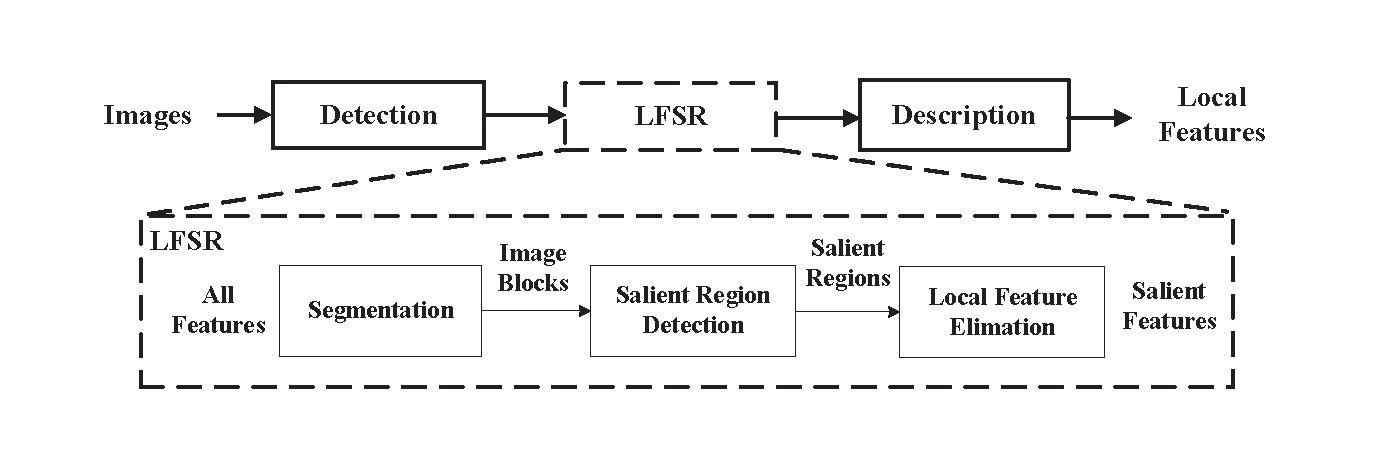
\includegraphics[width=5.0in]{images/fig-overview.eps}
\caption{An overview of Local Feature based Salient Region algorithm}
\label{fig:overview}
\end{figure*}

The basic motivation of {\sys} is to design a salient region detection algorithm, which can be used to optimize the obstacles of local feature-based algorithms and is easy to combined with those local feature based algorithms. Based on the observations in Section~\ref{subsec:observation}, we design and implement a local feature based salient region detection algorithm~({\sys}), which is efficient and easy to be combined with {\lfea}s.    

As shown in Figure \ref{fig:overview}, {\sys} works as a filter just between detection stage and description stage of a typical {\lfea}, where the input of {\sys} is detected feature points and output is concerned feature points for computing feature vectors. There exist two major stages in our algorithm.
\begin{inparaenum}[\itshape a\upshape)]
\item First, a segmentation step is performed on all local features to identify and partition multiple salient region in an image. 
\item Second, for each image segmentation, {\sys} computes that segmentation's salient region individually based on the distribution information of the local feature points in it.
\end{inparaenum}

\subsection{Local Feature Based Segmentation}
\label{sec:algorithm_segmentation}

According to Observation~\ref{itm:observation_2}, one image may have several salient regions which constructed as multiple clusters of local features. We solve this problem by using a simple image segmentation algorithm to divide the image into several blocks based on the distribution of local features. This segmentation performs scan operations on both the x axis and the y axis. In each scan, a cut-point may be found following these two constraints:

\begin{itemize}

  \item \textit{No local feature could be divided into multiple parts.} In {\lfea}s, scale information is computed to guaranteed scale invariant. Therefore, a local feature point is used to represent a region with a radius that equals its scale as shown in Figure~\ref{fig:segmentation}. When the image is partitioned, no segmentation should across a feature point.

  \item \textit{The cut point should not locate far away form the center.} Each scan is performed from the region center. When the scan goes far, for example 1/2 of the image width, the scan stops and declares that there is no valid cut in that scan. This constraint attends to keep segmentation balanced and avoid too large regions or too small regions.

\end{itemize}

A typical segmentation is shown in Figure~\ref{fig:segmentation}. The segmentation is started from the center of each axis, e.g. the dot lines in the figure. When a cut-point satisfying the above two constraints is found, The algorithm stops scanning and takes that cut-point as a valid image segmentation, e.g. the solid lines in the figure. After scanning on both the x axis and the y axis, at most four image regions are found in one segmentation.

Then this kind of segmentation will be performed recursively on each image regions. And a recursive segmentation should stop when following situations are satisfied:

\begin{itemize}

  \item \textit{No valid cuts are found.} When no valid cuts following the above two constraints are found, for example a scan exceeds its distance limit, on both x-axis and y-axis of a region, we should regard this region as a whole object and stop performing segmentation on it.

  \item \textit{Too few features exist in a region.} Some found regions may have no local feature or just one or two local features, like gray regions in Figure~\ref{fig:segmentation-2}. These regions will be marked as invalid, for they cannot hold one whole object, and no further computation will be performed on them.

  \item \textit{The number of segmentations exceeds the limitation.} It's possible that the recursive segmentation becomes too deep if there exists many dispersive points in that region. And actually it makes no sense to perform segmentation on these points, since they cannot be regarded as valid objects individually.

\end{itemize}

According to our evaluation, in most cases one run of segmentation is just enough, for almost no image has more than two major objects. Thus, it's possible to simplify this processing by performing segmentation only once in realistic scenarios.

\begin{figure}[!t]
\centering
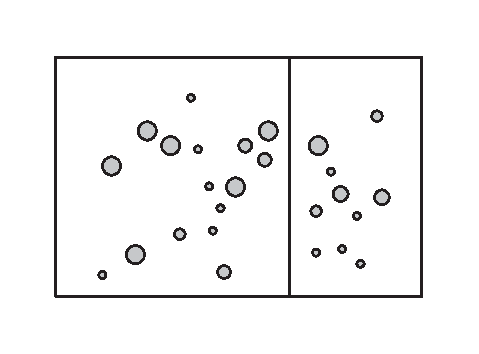
\includegraphics[width=2.5in]{images/fig-segmentation.eps}
\caption{Segmentation by scanning all local features on both the x-axis and y-axis. The scan starts form the dot lines and stops on the solid lines.}
\label{fig:segmentation}
\end{figure}

\begin{figure}[!t]
\centering
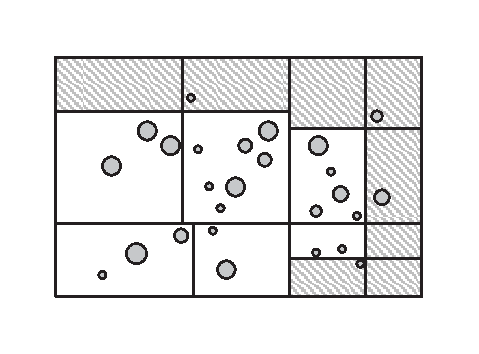
\includegraphics[width=2.5in]{images/fig-segmentation-2.eps}
\caption{Valid and invalid regions according after two runs of segmentations. White regions are valid and gray regions are invalid.}
\label{fig:segmentation-2}
\end{figure}

\subsection{Local Feature Based Detection}
\label{sec:algorithm_detection}

As discussed in Section~\ref{sec:algorithm_overview}, a precise salient region detection is not necessary for local feature reduction. Thus, {\sys} employs geometric meaning of local features to compute the salient region.

According to Observation~\ref{itm:observation_1}, the local features of one salient region locate near to each other while noises locating far away from them. To simplify this problem, we regard the geometric center of feature points as the center of salient region. Thus, the region center can be calculated like this:

{\begin{equation} \label{eq:center}
\left({x}_{c},{y}_{c} \right) = \frac{\sum_{i}^{N}\left({x}_{i},{y}_{i} \right)}{N}
\end{equation}}

Where $\left({x}_{c},{y}_{c} \right)$ means the geometric center of each local feature $\left({x}_{i},{y}_{i} \right)$ in that image segmentation.

After locating the center, we build the final salient region by expending the region as rectangle with a particular width-length ratio. This ratio should be consistent with the distribution of local features, since local features always locate following the shape of target objects. Approximately, this ratio can be considered to equal to the ratio of dispersion degree on x-axis and y-axis. For example, the bigger dispersion degree of local features on x-axis is, the bigger width-length ratio we will get. To compute the ratio of feature dispersions, we can divide the standard deviation of local feature position on x-axis by on y-axis:

{\begin{equation} \label{eq:ratio}
ratio = \sqrt{\frac{\sum_{i}^{N}\left ( x_{i}-x_{c} \right )^{2}}{\sum_{i}^{N}\left ( y_{i}-y_{c} \right )^{2}}}
\end{equation}}

Where $x_{i}$ and $y_{i}$ is a feature's position, while $x_{c}$ and $y_{c}$ is the center position computed by Equation~\ref{eq:center}. To get the final salient region, {\sys} grows the region size until the amount of local feature in it exceeds a desirable number, for example 50 percent of the original local features. As discussed in Observation \ref{itm:observation_3}, this threshold is important for providing a large enough salient region to avoid filtering local features on objects' edges and corners. In our evaluation, we find a ratio about 40\% is proper for most cases.

Combined with segmentation discussed in Section~\ref{sec:algorithm_segmentation}, the processing result will provide several candidate regions. According to Observation \ref{itm:observation_2}, we choose to pick up regions with most local features and regard them as final results.

\subsection{Local Feature Elimination}
\label{sec:algorithm_elimation}

With the knowledge of salient regions in an image, all features locate inside are kept for further computation, and all other features outside are just dropped. As a result, we get much fewer salient features in the local feature description stage, which can help to improve the whole algorithm's efficiency obviously.

\subsection{Cons and Pros}
\label{sec:algorithm_summary}

\textit{Cons:} As an approximate approach, {\sys} cannot handle two scenarios very well. First, images with very high texture background, such as images with grass and leaves in the background, have so many noisy local features around the concerned objects that our algorithm will detect error geometric centers on them. Second, {\sys} regards the object overlapped by others as a whole bigger object, leading to unnecessary larger salient regions and lower precision.

\textit{Pros:} {\sys} detects the salient regions very efficiently with only one mean value, two standard deviation, and a few additional loops to expand the detected region. Since these computations are only performed on local features, the cost should be very slight when integrated with a local feature descriptor. Actually, we find that our algorithm achieves an great performance advantage when compared to other precise salient region algorithms. 

